%!TEX root = ../thesis.tex
%*******************************************************************************
%****************************** Second Chapter *********************************
%*******************************************************************************

\chapter{SAT Solvers} \label{chap:solvers}

\ifpdf
    \graphicspath{{Chapter2/Figs/Raster/}{Chapter2/Figs/PDF/}{Chapter2/Figs/}}
\else
    \graphicspath{{Chapter2/Figs/Vector/}{Chapter2/Figs/}}
\fi


\section{Backtracking Based Algorithms}
Currently there are predominantly two classes of SAT solvers: those based on
backtracking search and those based on stochastic local search \cite{sat2018descriptions}. This chapter
will go over the two different classes, giving the algorithms that they are
based on followed by an overview of the details put into implementations of
a solver.

\subsection[DPLL]{Davis–Putnam–Logemann–Loveland} \label{sec:dpll}
One of the first SAT solving algorithms came from a desire to show the validity of
statements made in first order predicate logic. Here, we shall only concern ourselves
with the portion that is applicable to SAT formulas. Before introducing
Davis Putnam Logemann Loveland (DPLL),\nomenclature[z-DPLL]{DPLL}{Davis Putnam Logemann Loveland}
we shall consider its predecessor,
the Davis-Putnam procedure (DP)\cite{davis1960computing}.
\nomenclature[z-DP]{DP}{Davis Putnam procedure}
\nomenclature[x-equisat]{F $\approx$ G}{Boolean formulas F and G are equisatisfiable}
This procedure uses a resolution based approach and is based on 3 rules:

\begin{enumerate}
    \item (One Literal Clause Rule) If a formula has a clause containing a single unassigned literal,
    eliminate all clauses that contain this literal, and remove any occurrence of the negated
    literal from the remaining clauses.
    This is also referred to as unit propagation or boolean constraint propagation.
    A clause with only one unassigned literal, is sometimes referred to as a unit
    clause.
    \begin{equation*}
        (a) \land (a \lor b \lor c) \land (\neg a \lor \neg b \lor c) \approx (\neg b \lor c)
    \end{equation*}
    \item (Pure Literal Rule) If a variable in a formula occurs either only 
    as a literal in its positive form or only as a literal in its negative form.
    Then eliminate all clauses containing this literal.
    \begin{equation*}
        (a \lor b) \land (a \lor \neg b) \land (b \lor c) \approx (b \lor c)
    \end{equation*}
    \item (Resolution Rule) If there exist two clauses which share a variable where in one
    clause the literal is negated and in the other it is not. The two clauses can be replaced
    by a single clause containing the union of their literals excluding the shared variable.
    \begin{equation*}
        (a \lor x)\land(b \lor \neg x) \approx (a \lor b)
    \end{equation*}
\end{enumerate}

The simplified formulas that result from the application of these rules
are not necessarily equivalent to the original formulas, but they are
equisatisfiable. Therefore if a formula is simplified to the point it contains
no clauses then it is trivially satisfiable and the original formula is also
satisfiable. Observe that it is always possible to reduce a satisfiable formula
to the empty formula, since if the resolution rule cannot be applied then
the pure literal rule can remove all clauses.

To see this procedure in action consider checking whether the following
formula in CNF is satisfiable.

\begin{equation} \label{eq:DP_example}
    (a \lor b) \land (\neg a \lor b) \land (a \lor \neg b)
\end{equation}

As we see in Equation \ref{eq:DP_example}, we can apply the resolution rule
to the first two clauses. This yield the following simplification.

\begin{equation}
    (b) \land (a \lor \neg b)
\end{equation}

From here we see that we can apply the one literal clause rule to eliminate
the first clause. Note that the last clause will be simplified to just $(a)$.
Hence we can apply the one literal clause rule again to get the empty formula.
At this point the procedure finishes. Since we obtained the empty formula
we know that the original formula was satisfiable.

If a formula is unsatisfiable then the input formula will eventually
simplify to a formula containing the empty clause, which cannot be satisfied,
at this point the procedure would halt \cite{davis1960computing}.

Consider Equation \ref{eq:DP_example}, but with the added clause $(\neg a \lor \neg b)$.
This modified formula is now unsatisfiable and if we apply the same rules to
this new formula we will, instead of ending up with $(a)$, we will have
$(a) \land (\neg a)$. At this point, applying the pure literal rule to either
$a$ or $\neg a$ will leave one clause empty.

\subsubsection{Moving to DPLL}
An issue was that the
resolution rule could cause the size of clauses to increase rapidly. This
was an issue that prevented the procedure to implemented due to memory constraints.
The solution was to replace the resolution rule by the splitting rule which
can be stated as the following. Let $x$ be some variable in a formula, the formula
is inconsistent if and only if the formula is inconsistent when $x = \text{true}$ and
when $x = \text{false}$ \cite{davis1962machine}. This is theoretically equivalent
to the resolution rule, however this rule allowed for better memory usage in
practice.

The substitution of the resolution rule for the splitting rule forms the basis
for DPLL with most improvements focusing on finding efficient data
structures for implementing DPLL and on developing good heuristics for which
variable to branch on.

An important observation is that the splitting rule defines a tree with
the original formula as the root and the two children of the root are
the two formulas obtained from the splitting rule. Hence a formula is
satisfiable if and only if one of the leaves in the tree is satisfiable.
DPLL moves through the tree in a pre-order like fashion, this is called
chronological backtracking \cite{biere2009conflict}. However, note that
the order in which the tree is traversed and how the algorithm backtracks
does not affect the correctness of the algorithm as long as we can guarantee that every node in the tree will be visited eventually.
A run of DPLL on Equation \ref{eq:DP_example} can be seen in Figure \ref{fig:run_dpll}.

\begin{figure}
    \centering
    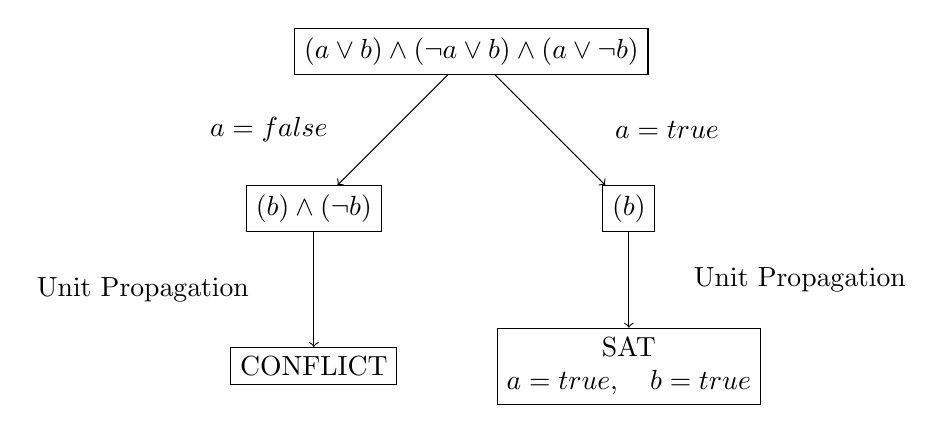
\begin{tikzpicture}
        \node[draw] (A) at (0,0)     {$(a \lor b) \land (\neg a \lor b) \land (a \lor \neg b)$};
        \node[draw] (B) at (-2,-2)   {$(b) \land (\neg b)$};
        \node[draw] (C) at (2,-2)    {$(b)$};
        \node[draw] (D) at (-2,-4) {CONFLICT};
        \node[draw, align=center] (E) at (2,-4)  {SAT \\ $a = \text{true},\quad b = \text{true}$};
        
        \draw[->]   (A) -- (B) node[midway, left=20pt] {$a = \text{false}$};
        \draw[->]   (A) -- (C) node[midway, right=20pt] {$a = \text{true}$};
        \draw[->]   (B) -- (D) node[midway, left=20pt] {Unit Propagation};
        \draw[->]   (C) -- (E) node[midway, right=20pt] {Unit Propagation};
    \end{tikzpicture}
    \caption{A run of DPLL on Equation \ref{eq:DP_example}}
    \label{fig:run_dpll}
\end{figure}

\subsection[CDCL]{Conflict Driven Clause Learning}
Recent competitive solvers are based on Conflict Driven Clause Learning (CDCL) \nomenclature[z-CDCL]{CDCL}{Conflict Driven CLause Learning}
\cite{SAT_Comp2017, sat2018descriptions}, such as Glucose.
CDCL builds on DPLL in a few ways, the key methods are as follows:

\begin{itemize}
    \item Derive new clauses when search yields a conflict \cite{marques1999grasp}.
    \item Use of efficient lazy data structures \cite{moskewicz2001chaff, ryan2004efficient}.
    \item Non-chronological backtracking \cite{marques1999grasp}.
    \item Restarting search \cite{gomes1998boosting, gomes2000heavy}
\end{itemize}

The structure of a CDCL solver without restarts can be seen in Algorithm \ref{alg:cdcl}.

\begin{algorithm}
\caption{Organisation of CDCL \cite{biere2009conflict, CDCL}}
\label{alg:cdcl}
\vspace{5pt}
\KwIn{CNF-SAT Formula $F$}
\KwOut{SAT or UNSAT}
\hrulefill\\

\nl $\alpha \gets \emptyset$ \\
\nl \If{unit\_propagation($F$, $\alpha$) == CONFLICT}
{
    \nl \Return{UNSAT} \\
}
\nl decision\_level $\gets 0$ \\
\nl \While{$\neg$ all\_variables\_assigned($F$, $\alpha$)}
{
    \nl $(x,v) \gets \text{pick\_branching\_variable}(F, \alpha)$ \\
    \nl decision\_level $\gets$ decision\_level $+ 1$ \\
    \nl $\alpha \gets \alpha \cup \{(x,v)\}$ \\
    \nl \If{unit\_propagation($F, \alpha$) == CONFLICT}
    {
        \nl $\beta \gets \text{conflict\_analysis}(F, \alpha)$ \\
        \nl \If{$\beta < 0$}
        {
            \nl \Return{UNSAT} \\
        }
        \nl \Else{
            \nl backtrack($F, \alpha, \beta$) \\
            \nl decision\_level $\gets \beta$ \\
        }
    }
}
\nl \Return{SAT}
\end{algorithm}

In Algorithm \ref{alg:cdcl} $\alpha$ refers to the set of assignments, where
each assignment is represented as a tuple $(x, v)$ where $x$ is a variable
and $v \in \{\text{false}, \text{true}\}$ is the value. The unit propagation
function call executes the one literal clause rule from Section \ref{sec:dpll}.
Pick branching variable chooses which variable to branch on and gives it a value.
Choice of heuristics for which variable to select is motivated mostly by which
features can be computed efficiently \cite{lewis2005speedup, moskewicz2001chaff}.

Backtrack takes in a parameter $\beta$, which indicates the decision level to
backtrack to. This means that search happens in a non-chronological fashion.
The level to backtrack to is decided by the conflict analysis function.
% This function looks at which clauses clauses the contradiction to occur
% and finds a clause implied by those clauses and adds it to the formula.
% The amount to backtrack by depends on what decision level the variables
% in the learned clause were assigned. One scheme involves always backtracking
% to the decision level of the most recently assigned variable \cite{biere2009conflict}.

\subsubsection{Conflict Analysis}
The most characteristic part of CDCL is the clause learning that results from the clause
analysis process. There are slight variants of this procedure, but we will cover the most
common variations popularised in GRASP \cite{marques1999grasp} and Chaff \cite{moskewicz2001chaff}.

For a particular partial assignment $\alpha$, we use decision level to mean the order that
a given variable was assigned by the \texttt{pick\_branching\_variable} routine. For
variables that were assigned via the \texttt{unit\_propagation} routine, they inherit the
highest decision level of the other variables in the clause. We consider a variable that
is assigned via \texttt{unit\_propagation} to be implied by the other variables in the unit clause.
Since \texttt{unit\_propagation} may lead to more clauses becoming unit, we can construct a directed
acyclic graph of implications. We call this graph the implication graph.

Consider the following boolean formula:
\begin{align}
    &(\neg x_1 \lor x_2 \lor x_4) \land (x_2 \lor \neg x_3 \lor \neg x_5) \land (\neg x_4 \lor x_5 \lor x_6) \nonumber \\
    \land &(\neg x_6 \lor x_7) \land (\neg x_3 \lor \neg x_6 \lor \neg x_8) \land (\neg x_7 \lor x_8) \label{eq:impl_ex}
\end{align}
For example, say that \texttt{pick\_branching\_variable} first assigns $x_1 = \text{true}$ at decision level 1, then
$x_3 = \text{true}$ at decision level 2 and then $x_2 = \text{false}$ at decision level 3. At this point, the first
two clauses in Equation \ref{eq:impl_ex} are unit clauses and applying \texttt{unit\_propagation} will lead to a conflict.
The resulting implication graph can be seen in Figure \ref{fig:implication_graph}. Each vertex represents an assignment
or a conflict and there is a directed edge from one vertex to another if that assignment implies the other via unit
propagation. For example, in Figure \ref{fig:implication_graph} there is an edge from $x_1 = \text{true}$ and $x_2 = \text{false}$
to $x_4 = \text{true}$ because the first two assignments make the clause $(\neg x_1 \lor x_2 \lor x_4)$ a unit clause which
implies $x_4 = \text{true}$. There are also edges from $x_7 = \text{true}$ and $x_8 = \text{false}$ to a conflict vertex since
these two assignments leave the clause $(\neg x_7 \lor x_8)$ unsatisfied. Each edge is labelled with the clause
that caused the implication.

\begin{figure}
    \centering
    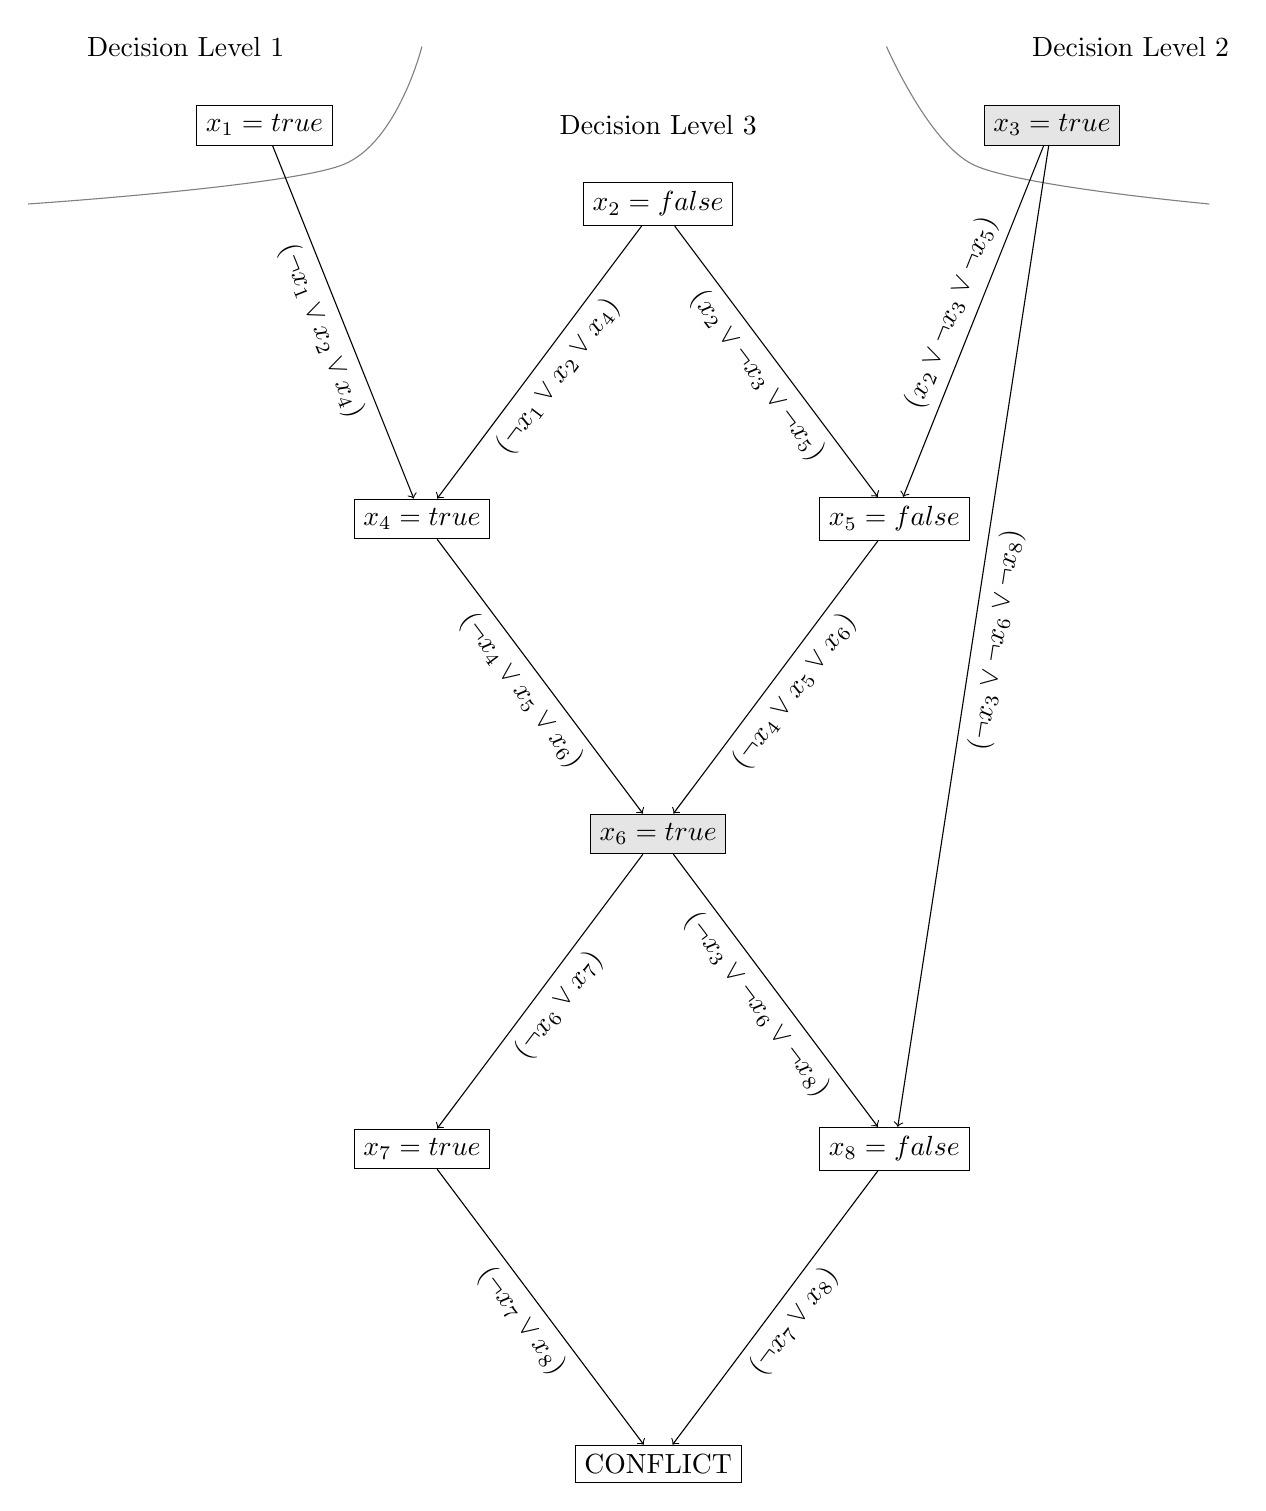
\begin{tikzpicture}
        \node[draw] (x1) at (-5, 1) {$x_1 = \text{true}$};
        \node[draw] (x2) at (0, 0) {$x_2 = \text{false}$};
        \node[draw, fill=black!10] (x3) at (5, 1) {$x_3 = \text{true}$};
        \node[draw] (x4) at (-3, -4) {$x_4 = \text{true}$};
        \node[draw] (x5) at (3, -4) {$x_5 = \text{false}$};
        \node[draw, fill=black!10] (x6) at (0, -8) {$x_6 = \text{true}$};
        \node[draw] (x7) at (-3, -12) {$x_7 = \text{true}$};
        \node[draw] (x8) at (3, -12) {$x_8 = \text{false}$};
        \node[draw] (k) at (0, -16) {CONFLICT};
        
        \draw[gray] plot [smooth] coordinates {(-8, 0) (-4, 0.5) (-3, 2)};
        \draw[gray] plot [smooth] coordinates {(7, 0) (4, 0.5) (2.9, 2)};
        \node[] (dl1) at (-6, 2) {Decision Level 1};
        \node[] (dl2) at (6, 2) {Decision Level 2};
        \node[] (dl3) at (0, 1) {Decision Level 3};
        
        \path[->] (x1) edge node[below, sloped] {$(\neg x_1 \lor x_2 \lor x_4)$} (x4);
        \path[->] (x2) edge node[below, sloped] {$(\neg x_1 \lor x_2 \lor x_4)$} (x4);
        \path[->] (x2) edge node[below, sloped] {$(x_2 \lor \neg x_3 \lor \neg x_5)$} (x5);
        \path[->] (x3) edge node[above, sloped] {$(x_2 \lor \neg x_3 \lor \neg x_5)$} (x5);
        \path[->] (x3) edge node[below, sloped] {$(\neg x_3 \lor \neg x_6 \lor \neg x_8)$} (x8);
        \path[->] (x4) edge node[below, sloped] {$(\neg x_4 \lor x_5 \lor x_6)$} (x6);
        \path[->] (x5) edge node[below, sloped] {$(\neg x_4 \lor x_5 \lor x_6)$} (x6);
        \path[->] (x6) edge node[below, sloped] {$(\neg x_6 \lor x_7)$} (x7);
        \path[->] (x6) edge node[below, sloped] {$(\neg x_3 \lor \neg x_6 \lor \neg x_8)$} (x8);
        \path[->] (x7) edge node[below, sloped] {$(\neg x_7 \lor x_8)$} (k);
        \path[->] (x8) edge node[below, sloped] {$(\neg x_7 \lor x_8)$} (k);
    \end{tikzpicture}
    \caption{Implication graph for Equation \ref{eq:impl_ex} for a partial assignment to $x_1, x_2, x_3$.
    First UIP is shaded grey}
    \label{fig:implication_graph}
\end{figure}

The \texttt{conflict\_analysis} routine will construct this implication graph and then apply
a number of resolution steps to obtain the learned clause. Define a resolution operator $\odot$ for
two clauses $C_1$ and $C_2$ with a unique variable $x_r$ such that $\neg x_r \in C_1$ and $x_r \in C_2$ or
vice versa, then $C_1 \odot C_2 = (C_1 \cup C_2) \setminus \{x_r, \neg x_r\}$ i.e. a clause containing
all literals in $C_1$ and $C_2$ excluding $x_r$ and $\neg x_r$. \texttt{conflict\_analysis} then begins by
taking the clause that caused the conflict (in this example $(\neg x_7 \lor x_8)$) and applying the resolution
operator with this clause and a clause that implied one of the literals in the first clause. In our example
the first resolution step could be either $(\neg x_7 \lor x_8) \odot (\neg x_6 \lor x_7) = (\neg x_6 \lor x_8)$ or 
$(\neg x_7 \lor x_8) \odot (\neg x_3 \lor \neg x_6 \neg x_8) = (\neg x_3 \lor \neg x_6 \lor \neg x_7)$.
A full set of resolution steps using the example from Equation \ref{eq:impl_ex} can be seen in Table \ref{tab:resolutions}.
Since $\forall C_1, C_2 \in F : C_1 \odot C_2 \approx C_1 \land C_2$ then $F \approx F \cup \{C_1 \odot C_2\}$. This means
that we can take any clause from Table \ref{tab:resolutions} and add it to Equation \ref{eq:impl_ex} without changing
its satisfiability.

\begin{table}[]
    \centering
    \begin{tabular}{l l}
    \toprule
        Step & Resolution \\
    \midrule
        1 & $(\neg x_7 \lor x_8) \odot (\neg x_6 \lor x_7) = (\neg x_6 \lor x_8)$ \\
        2 & $(\neg x_6 \lor x_8) \odot (\neg x_3 \lor \neg x_6 \lor \neg x_8) = (\neg x_3 \lor \neg x_6)$ \\
        3 & $(\neg x_3 \lor \neg x_6) \odot (\neg x_4 \lor x_5 \lor x_6) = (\neg x_3 \lor \neg x_4 \lor x_5)$ \\
        4 & $(\neg x_3 \lor \neg x_4 \lor x_5) \odot (x_2 \lor \neg x_3 \lor \neg x_5) = (x_2 \lor \neg x_3 \lor \neg x_4)$ \\
        5 & $(x_2 \lor \neg x_3 \lor \neg x_4) \odot (\neg x_1 \lor x_2 \lor x_4) = (\neg x_1 \lor x_2 \lor \neg x_3)$ \\
    \bottomrule
    \end{tabular}
    \caption{Resolution steps for Equation \ref{eq:impl_ex} with partial assignments to $x_1, x_2, x_3$}
    \label{tab:resolutions}
\end{table}

\nomenclature[z-UIP]{UIP}{Unit Implication Point}

There are different options for how many resolution steps to perform, however, a guiding principle is that the learned clause
should be as short as possible and should remain a unit clause after backtracking.
The most common approach is to stop at what is called the first Unit Implication Point (UIP) \cite{biere2009conflict}, which is the first point
at which there is only one literal in a learned clause that has the highest decision level. In Table \ref{tab:resolutions}
this occurs at step 2, since in the clause $(\neg x_3 \lor \neg x_6)$ only $x_6$ has decision level 3 while $x_3$
has decision level 2.
Note that if we look at the literals in a clause obtained by any number of resolution steps, the corresponding vertices
in the implication graph form a vertex separator, separating the side of the graph containing the conflict vertex
and the side containing the variables in the assignments made by \texttt{pick\_branching\_variable}. 
Therefore, we can interpret a UIP as a clause where the variable with the highest decision level
is a dominator for the variable most recently assigned by \texttt{pick\_branching\_variable}
with respect to the conflict vertex. This can be seen in Figure \ref{fig:implication_graph} as all paths from $x_2 = \text{false}$
to the conflict vertex must pass through $x_6 = \text{true}$.

The amount to backtrack by (given by $\beta$ in Algorithm \ref{alg:cdcl}) also varies from solver to solver
and most often depends on how inexpensive backtracking is given the datastructures used by the solver.
However, most modern solvers now use lazy datastructures which make it cheap to backtrack. For these
solvers a common approach is to backtrack until just before the learned clause no longer is a unit clause.
In the example given in Equation \ref{eq:impl_ex}, the learned clause was $(\neg x_3 \lor \neg x_6)$. As long
as $x_3$ remains assigned then the learned clause will be a unit clause, and $x_3$ was assigned at decision level 2,
so we can backtrack to decision level 2. In general we can backtrack to the second highest decision level in the
learned clause. This is the backtracking method used by Chaff \cite{moskewicz2001chaff}.
We can guarantee completeness because, since the learned clauses prevent the solver from exploring
the same assignment twice.

\subsubsection{Performance}

\begin{figure}
    \centering
    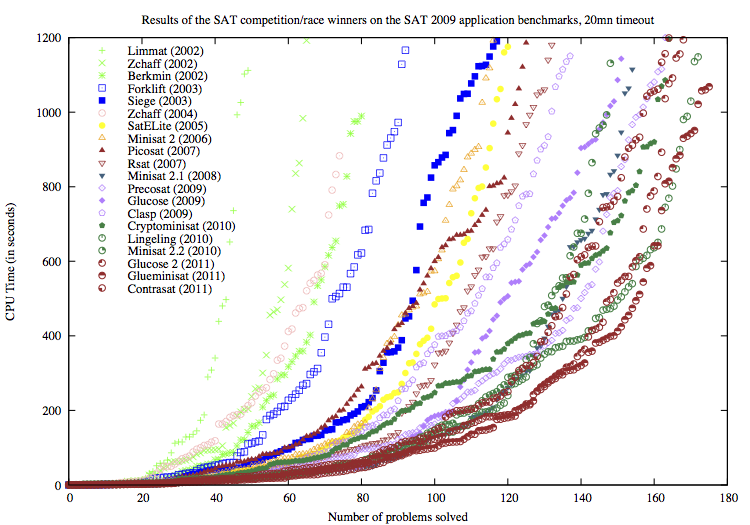
\includegraphics[scale=1]{sat_performance2012.png}
    \caption{Number of sat problems taken from the
    2009 SAT competition that were solved by various solvers
    with a 20 minute timeout \cite{sat2009theory}}
    \label{fig:sat_perf}
\end{figure}

In figure \ref{fig:sat_perf} we can see the number of solved instances of practical
sat benchmarks submitted to the 2009 SAT competition by various different solvers
\cite{sat2009theory}. Notably
more recent solvers, whilst still demonstrating exponential scaling behaviour are
able to solve significantly more problems than prior solvers.

For the 2018 SAT competition the benchmarks were taken from various different domains:
\cite{sat2018descriptions}

\begin{itemize}
    \item Proving the existence of a nonce for blockchain mining algorithms.
    \item Searching for a unit-distance graph with chromatic number 6 and k-colourability of graphs.
    \item Verifying simple floating-point programs.
    \item Cryptanalysis.
    \item Time-Slot allocation problems with optimal preference satisfaction
\end{itemize}

\subsection{Glucose}
Glucose is an efficient implementation of CDCL that has featured prominently
in many SAT competitions \cite{audemard2009glucose} building on top of MiniSAT \cite{een2003extensible}.
Glucose implements a few additional
features on top of CDCL, most prominently it implements new clause deletion policies
which help control the memory usage of the learned clauses generated by
the conflict analysis. These deletion policies expand on those used in the BerkMin solver \cite{goldberg2007berkmin},
going beyond analysing clauses just by size and how close they are to being a unit clause \cite{dechter1990enhancement, bayardo1997using}.

These policies were established in work by Audemard et al. where it is observed that
the decision level at which conflicts are encountered
tends to decrease as the solver progresses \cite{audemard2009predicting},
although this effect was only observed for ``industrial'' SAT instances.
This means that the solver is able to find conflicts faster over time, i.e.
it is assigning many variables via unit propagation. Additionally, this allows
for a crude estimate of when the solver will terminate.
Audemard et al. then devise a metric called the ``Literal
Block Distance'' (LBD) \nomenclature[z-LBD]{LBD}{Literal Block Distance}
which is the number of distinct decision levels in a clause
for a given assignment and show that when keeping only clauses with low LBD
the observation that decision levels decrease still holds. This suggests
that these clauses are the most important for allowing the solver to
spend significant time executing unit propagation.
Applying this deletion policy, around 93\% of learned clauses were deleted \cite{audemard2009glucose}.
However, since the learned clauses are needed for guaranteeing completeness, Glucose
is not complete.

Of practical note is that the Glucose solver is particularly
amenable to paralellisation and remains one of the most
competitive parallel solvers \cite{audemard2018glucose}.

\section{Stochastic Local Search Algorithms}
A different family of algorithms to backtracking algorithms is local search algorithms
which are based on the idea of randomly choosing an assignment and then making
small adjustments to assignment in order to try and find a satisfying assignment.
We will cover an important algorithm,
namely Sch\"oning's algorithm \cite{schoning1999probabilistic}, and then consider
WalkSat, a solver based on similar principles.

\subsection{Sch\"oning's Algorithm}

An interesting $k$-SAT algorithm that is able to beat the $\mathcal{O}^*(2^n)$
complexity for bounded $k$ is Sch\"oning's algorithm seen in Algorithm \ref{alg:schoning}.
Given that a satisfying assignment exists it will be found in expectation after
$(2 - \frac{2}{k})^n$ runs of Sch\"oning's algorithm \cite{schoning1999probabilistic}.
Hence the expected running time is $\mathcal{O}^*((2 - \frac{2}{k})^n)$.

\begin{algorithm}
\caption{Sch\"oning's Algorithm for $k$-SAT}\label{alg:schoning}
\vspace{5pt}
\KwIn{$k$-SAT instance, $F$}
\KwOut{Instance is satisfiable or not}
\hrulefill \\
\nl Guess initial assignment \\
\nl \For{$i \in \{1, \dots, 3n\}$}{
    \nl \If{$F$ is Satisfied}{
        \nl \Return{Accept} 
    }
    \nl \Else{
        \nl flip a random variable in an unsatisfied clause \\
    }
}
\end{algorithm}

\subsubsection{Analysis of Sch\"oning's Algorithm}
For the sake of brevity, we will only consider the case where $k=3$.
Since we require that there is at least one satisfying assignment let $\alpha^*$
be one such satisfying assignment. Let $\alpha$ be the assignment guessed in
the first line and let $d$ be the Hamming distance between $\alpha$ and $\alpha^*$,
i.e. $H(\alpha, \alpha^*) = d$ the number of variables in which they differ. The probability of guessing
an assignment $\alpha$ which differs by exactly $d$ variables from $\alpha^*$ is given by the following expression,
where $n$ is the number of variables.

\begin{equation}
    2^{-n}\binom{n}{d}
\end{equation}

If the algorithm flips a variable in which $\alpha$ and $\alpha^*$ differ, then
we call this a step towards the solution, i.e. $H(\alpha, \alpha^*)$ decreases by 1. Conversely, if they do not differ then
we call this a step away from the solution, i.e. $H(\alpha, \alpha^*)$ increases by 1.
%Let $T$ be the total number of steps,
%if a run of the algorithm where to find a satisfying assignment then we
%must have that the number of steps towards the solution must be
%$\frac{T + d}{2}$ and steps away must be $\frac{T - d}{2}$

Consider the probability of making $2d$ steps towards the solution
and $d$ steps away in the first $3d$ steps. It is clear that this will reach
$\alpha^*$ and since $d \leq n$, then the total number of steps 
will not be greater than $3n$. Since, in an unsatisfied clause,
at least one variable is different between $\alpha$ and $\alpha^*$, then when
the algorithm flips a random variable in that clause the probability of it
being one where the assignments are different is $\frac{1}{3}$. Hence,
the probability of making $2d$ toward the solution and $d$ steps away in the
first $3d$ steps is given by the following expression.

\begin{equation}
    \binom{3d}{d} \Big( \frac{1}{3} \Big)^{2d} \Big( \frac{2}{3} \Big)^d
\end{equation}

Hence to find the probability that the algorithm finds a satisfying solution
we simply have combine this with the probability of guessing a first assignment
that has Hamming distance of exactly $d$, and sum over all possible values of $d$.

\begin{equation} \label{eq:p_find_assignment}
    \mathrm{Pr}[\text{Find satisfying assignment}] = \sum_{d=0}^{n} 2^{-n}\binom{n}{d}\binom{3d}{d} \Big( \frac{1}{3} \Big)^{2d} \Big( \frac{2}{3} \Big)^d
\end{equation}

To simplify Equation \ref{eq:p_find_assignment} it will be helpful to consider
a lower bound of $\binom{3d}{d}$. To do this we will use Stirling's approximation
of the factorial:

\begin{equation} \label{eq:stirling_fac}
    n! \sim \sqrt{2\pi n} \Big( \frac{n}{e} \Big)^n
\end{equation}

Using Equation \ref{eq:stirling_fac} we can derive an approximation as follows.

\begin{align*}
    \binom{3d}{d} &= \frac{(3d)!}{(2d)! \cdot d!} \\[5pt]
    &\sim \frac{\sqrt{6 \pi d}\Big(\frac{3d}{e}\Big)^{3d}}{\sqrt{4\pi d} \Big( \frac{2d}{e} \Big)^{2d}\sqrt{2\pi d} \Big( \frac{d}{e} \Big)^d} \\[5pt]
    &\sim \frac{\sqrt{3}}{2\sqrt{\pi d}} \cdot \frac{3^{3d}}{2^{2d}}
\end{align*}

Since $n \geq d$ we replace $\sqrt{d}$ with $\sqrt{n}$ to simplify the analysis.
Then since the binomial coefficient is always strictly positive then what
remains is to choose a sufficiently large constant $\delta$
such that we have for $d \geq 0$:

\begin{equation} \label{eq:binom_bound}
    \binom{3d}{d} \geq \frac{1}{\delta \sqrt{n}} \cdot \frac{3^{3d}}{2^{2d}}
\end{equation}

Combining Equations \ref{eq:p_find_assignment} and \ref{eq:binom_bound} we get
a lower bound on the probability of finding a satisfying assignment.

\begin{align*}
    \mathrm{Pr}[\text{Find satisfying assignment}] &\geq \sum_{d=0}^{n} 2^{-n}\binom{n}{d} \frac{1}{\delta \sqrt{n}} \cdot \frac{3^{3d}}{2^{2d}} \Big( \frac{1}{3} \Big)^{2d} \Big( \frac{2}{3} \Big)^d \\[5pt]
    %&\geq \frac{2^{-n}}{\delta \sqrt{n}}\sum_{d=0}^{n} \binom{n}{d}\frac{3^{3d}}{2^{2d}} \frac{1}{3^{2d}} \frac{2^d}{3^d} \\[5pt]
    &\geq \frac{2^{-n}}{\delta \sqrt{n}}\sum_{d=0}^{n} \binom{n}{d}\frac{1}{2^{d}} \\[5pt]
    &\geq \frac{2^{-n}}{\delta \sqrt{n}}\Big( 1 + \frac{1}{2} \Big)^n \\[5pt]
    &\geq \frac{1}{\delta \sqrt{n}}\Big( \frac{3}{4} \Big)^n \\[5pt]
\end{align*}

Repeatedly running Algorithm \ref{alg:schoning} defines a geometric sequence.
Therefore, the expectation of the number of runs required to find the satisfying
assignment is given by

\begin{equation}
    \mathbb{E}[\text{\#runs}] = \frac{1}{\mathrm{Pr}[\text{Find satisfying assignment}]} \leq \delta\sqrt{n}\Big( \frac{4}{3} \Big)^n
\end{equation}

Hence the time complexity can be written as $\mathcal{O}^*(1.334^n)$.

\subsection{WalkSat}
WalkSat is an solver similar to Sch\"oning's algorithm that is inspired
by GSAT \cite{selman1992new, selman1994noise, selman1993local} and by ideas laid forth by Papadimitriou \cite{papadimitriou1991selecting}. The main difference between
WalkSat and Sch\"oning's algorithm is that it employs a semi-greedy
strategy when deciding which variable to flip in an unsatisfied clause.

With some probability $p$ WalkSat will flip a random variable, but
with probability $1 - p$ WalkSat will flip the variable that minimises
the number of clauses that become unsatisfied. The parameter $p$
is often called the noise parameter and optimal choice of $p$ depends
on the structure of the formula being tested. Therefore, modern improvements
have attempted to adapt $p$ automatically to each instance \cite{hoos2002adaptive}.

\begin{table}
    \centering
    \begin{tabular}{l l c c c}
    \toprule
        \multicolumn{2}{l}{Formula} & DP Time & GSAT Time & WalkSat Time \\
        \#Vars & \#Clauses & & & \\
        \midrule
        708 & 1702 & * & 0.081 & 0.013 \\
        649 & 1562 & * & 0.058 & 0.014 \\
        8704 & 32316 & * & 94.1 & 1.0 \\
        8432 & 31310 & * & 456.6 & 0.7 \\
        300 & 730 & 23096 & 0.009 & 0.002 \\
        125 & 310 & 1.4 & 0.009 & 0.001 \\
        \bottomrule
    \end{tabular}
    \caption[Comparing DP, GSAT and WalkSat]
    {Comparing solution times of an implementation of
    the Davis Putnam procedure (DP) with GSAT and WalkSat 
    (time in seconds) \cite{selman1993local}}
    \label{tab:walksat_times}
\end{table}

WalkSat is an efficient solver that is able to tackle SAT instances with a large
number of variables and clauses, and is able to find solutions to instances
where an efficient implementation of the Davis Putnam procedure was unable
to a find a solution. An overview of solution times for a few SAT benchmark
problems from 1993 is seen in Table \ref{tab:walksat_times}.